\section{\AP{}Introduction}
\label{sec:intro}

\subsection{\AP{}Graph Databases}

"Graph databases" have gained significant attention due to their ability to efficiently model and manage complex, interconnected data. Unlike traditional relational databases, they model data as entities connected by edges that represent relationships. This structure facilitates the analysis of highly interconnected data, where the topology of the connections is as crucial as the data itself, making them particularly well-suited for use cases like biology, social networks, banking, recommendation systems, and fraud detection. We refer the reader to \cite{Barcelo-pods13,DBLP:journals/sigmod/Wood12,survey-graphdbs2017} for surveys on the foundations and applications of graph databases.


% \footnote{This paragraph was partially written with the help of ChatGPT.}
% The growing need to handle large-scale,
% dynamic datasets with intricate relationships motivates further exploration of this model,
% as it provides both scalability and performance benefits in contexts where relationships between data points are central.

\AP ""Graph databases"" are abstracted as edge-labelled directed graphs
$G = \langle \vertex{G}, \edges{G} \rangle$, 
where nodes of $\intro*\vertex{G}$ represent entities and labelled edges $\intro*\edges{G} \subseteq \vertex G \times \A \times \vertex G$
represent relations between these entities, with $\A$ being a fixed finite alphabet.
For instance, \Cref{fig:example-graph-database} depicts a "graph database",
whose nodes are authors and papers, on the alphabet
$\A = \{\text{\color{wrote}wrote},\,\text{\color{advised}advised}\}$.
Edges $x \atom{\wrote} y$ indicate that the person $x$ wrote the paper $y$,
while edges $x \atom{\advised} y$ indicate that person $x$ was
the Ph.D. advisor of person $y$.

\begin{figure}[ht]
    \centering
    \begin{tikzpicture}
        \node (a1) {author$_1$};
        \node (a2) [right = of a1] {author$_2$};
        \node (a3) [right = of a2] {author$_3$};
        \node (a4) [right = of a3] {author$_4$};
        \node (a5) [right = of a4] {author$_5$};
        \node (p1) [below = 2.5em of a2] {paper$_1$};
        \node (p2) [below = 2.5em of a3] {paper$_2$};
        \node (p3) [below = 2.5em of a4] {paper$_3$};

        \draw[wrote] (a1) edge[->] node[fill=white] {\footnotesize wrote} (p1)
            (a2) edge[->] node[fill=white] {\footnotesize wrote} (p1)
            (a2) edge[->] node[fill=white] {\footnotesize wrote} (p2)
            (a3) edge[->] node[fill=white] {\footnotesize wrote} (p2)
            (a4) edge[->] node[fill=white] {\footnotesize wrote} (p3)
            (a5) edge[->] node[fill=white] {\footnotesize wrote} (p3);
        \draw[advised] (a4) edge[->, bend right=40] node[fill=white] {\footnotesize advised} (a3)
            (a5) edge[->, bend right=40] node[fill=white] {\footnotesize advised} (a4);
    \end{tikzpicture}
    \caption{%
        \AP\label{fig:example-graph-database}%
        A "graph database" with eight nodes and eight edges on a two-letter alphabet.
    }
\end{figure}

\AP Being a subclass of relational databases, "graph databases" can be queried by the
predominant query language of ""conjunctive queries"", "aka" "CQs", 
which consists of the closure under projection---"aka" existential quantification---of conjunctions of atoms of the form $x \atom{a} y$
for some letter $a \in \A$. For instance, the "conjunctive query"
\[
    \gamma_1(x, y) = x \atom{\wrote} z
        \land y \atom{\wrote} z    
\]
returns, when "evaluated" on the "graph database" $G$
defined in \Cref{fig:example-graph-database}, all pairs of nodes $(u, v)$ such that $u$ is a co-author
of $v$. Each variable not appearing in the left-hand side of 
the definition of a "conjunctive query" (in this example, $z$) is implicitly 
existentially quantified. 
Note that, to the cost of losing the information of which variable is existentially quantified, every "CQ"
can be seen as a "graph database", where each variable is a node, and each atom is an edge; 
hence, we sometimes use "graph database" terminology for "CQs".

The expressive power of "CQs" is somewhat limited, since
"CQs" cannot express, for example, transitive closure.
Since the ability to navigate paths is of importance in many "graph database" 
scenarios, most modern graph query languages support, as a central querying mechanism,
"conjunctive regular path queries", or "CRPQs" for short. 
In particular, "CRPQs" form the core navigational mechanism of the new ISO standard Graph Query Language (GQL) \cite{isoGQL} and the SQL extension for querying graph-structured data SQL/PGQ \cite{isoPGQ} (see also \cite{DBLP:conf/icdt/FrancisGGLMMMPR23,DBLP:conf/pods/FrancisGGLMMMPR23}).

"CRPQs" are 
defined analogously to "conjunctive queries", except that their atoms are now of the form 
$x \atom{L} y$ where $L$ is an arbitrary regular language over the alphabet $\A$. For 
instance the "evaluation" of the "CRPQ"
\[
    \gamma_2(x, y) = x \atom{\wrote} z
        \land z' \atom{\wrote} z 
        \land y \atom{({\advised})^*} z'
\]
on $G$ yields every pair of persons $(u,v)$ such that $u$ is a co-author of a
``scientific descendant'' of $v$. 

\AP Formally, a ""CRPQ"" $\gamma$ is defined as a tuple $\bar z = (z_1,\hdots,z_n)$
of ""output variables"", "aka" \reintro{free variables},\footnote{For technical reasons (see the definition of "equality atoms") we allow for a variable to appear multiple times.}
together with a conjunction of ""atoms"" of the form
$\bigwedge_{j=1}^m x_j \atom{L_j} y_j$, where each $L_j$ is a regular language and where $m \geq 0$.
The set of all variables occurring in $\gamma$, namely\footnote{We neither assume 
disjointness nor inclusion between $\{z_1,\hdots,z_n\}$ and $\{x_1,y_1,\hdots,x_m,y_m\}$}
$\{z_1,\hdots,z_n\}\cup\{x_1,y_1,\hdots,x_m,y_m\}$, is denoted by
$\intro*\vars(\gamma)$.
Given a "database" $G$, we say that a tuple of nodes $\bar u = (u_1,\hdots,u_n)$
\AP""satisfies"" $\gamma$ 
on $G$ if there is a mapping
$\fun\colon \vars(\gamma) \to \vertex{G}$ such that $u_i = \fun(z_i)$ for all
$1 \leq i \leq n$, and for each $1 \leq j \leq m$,
there exists a path from $\fun(x_i)$ to $\fun(y_i)$ in $G$, labelled by
a word from $L_i$ (if the path is empty, the label is $\epsilon$). The \AP""evaluation"" of $\gamma$ on $G$ is then the set of all tuples that "satisfy" $\gamma$.
%
For example, $(\text{author}_2, \text{author}_5)$ "satisfies" $\gamma_2$ 
on the "graph database" $G$ of \Cref{fig:example-graph-database} via
the function that maps $x$ to $\text{author}_2$, $y$ to $\text{author}_5$,
$z$ to $\text{paper}_2$, and $z'$ to $\text{author}_3$.

\AP
The language of "CRPQ" can be extended to navigate edges in both directions. 
\knowledgenewrobustcmd{\Gpm}{\cmdkl{G^\pm}}
Consider the expanded database $\intro*\Gpm$ obtained from $G$ by 
% keeping the same vertices, copying the edges of $G$, and 
adding, for every edge $x \atom{a} y$ in $G$, an extra edge $y \atom{a^-} x$.
We obtain a graph database on the alphabet $\intro*\Aext = \A \cup \A^-$ where
$\A^- = \set{a^- \mid a \in \A}$. We then define the syntax of
a \AP""CRPQ with two-way navigation"", or \reintro{C2RPQ}, as a "CRPQ" on the alphabet $\Aext$.
Its \reintro{evaluation} is defined as the "evaluation" of the "CRPQ" on $\Gpm$.
For instance, the "evaluation" of the "C2RPQ"
\[
    \gamma_3(x, y) = x \atom{({\wrote}\cdot{\wrote}^-)^*} y
\]
on the "graph database" of \Cref{fig:example-graph-database} returns all pairs of
individuals linked by a chain of co-authorship.
It includes $(\text{author}_1, \text{author}_3)$ or $(\text{author}_1, \text{author}_1)$
but not $(\text{author}_1, \text{author}_4)$.
%
\AP If a query has no "output variables" we call it ""Boolean"", and
its "evaluation" can either be the set $\set{()}$, in which case we say that $G$
\reintro{satisfies} the query, or the empty set $\set{}$. For example, $G$ "satisfies" the
"Boolean CRPQ"
\[\gamma_4() = x \atom{\wrote} y\]
if, and only if, the database contains one author together with one paper they wrote.

To simplify proofs, we assume that all the regular languages are described via 
non-deterministic  finite automata (NFA) instead of regular expressions,
which does not affect any of our complexity bounds.
However, for readability all our examples will be given in terms of regular expressions.
We denote the set of "atoms" of a "C2RPQ" $\gamma$ by \AP$\intro*\atoms\gamma$, and by 
$\intro*\nbatoms{\gamma}$ we denote its number of "atoms", "ie", $|\atoms\gamma|$.
Moreover, we denote by $\intro*\size{\gamma}$ the sum of its number of "atoms" with
the sum of the size of NFAs used to describe $\gamma$.


\AP Finally, a ""union of CQs"" (\reintro{UCQs}) (resp.\ ""union of CRPQs"" (\reintro{UCRPQs}), resp.\ ""union of C2RPQs"" (\reintro{UC2RPQs}))  
is defined as a finite set of "CQs" (resp.\ "CRPQs", resp.\ "C2RPQs"), whose
tuples of "output variables" have all the same arity. 
\AP
A ""subquery"" of a "C2RPQ" $\gamma$ is any "C2RPQ" resulting from removing some "atoms" (possibly none) from $\gamma$. A \reintro{subquery} of  "UC2RPQ" is a union of "subqueries" of the "C2RPQs" therein.
The "evaluation" of a union is defined as the union of its "evaluations", for instance the following "UCQ"
\begin{align*}
    \Gamma_5 & = \gamma_{5}^1(x, y) \lor \gamma_{5}^2(x, y) \\
    & \text{ where }
    \gamma_{5}^1(x, y) = x \atom{\wrote} y %\\
    \text{ and }
    \gamma_{5}^2(x, y) = x \coatom{\advised} z \land
        z \atom{\wrote} y
\end{align*}
"evaluates" to the set of pairs $(x,y)$ such that $y$ is a paper written by either $x$
or their advisor.
We naturally extend the notations $\nbatoms{-}$ and $\size{-}$ to "unions@UC2RPQs".
\AP ""Infinitary unions"" are defined analogously, except
that we allow for potentially infinite unions. We often use a set notation to denote the union, especially for "infinitary unions".

For a more detailed introduction to "CRPQs", we refer the reader to \cite{DBLP:conf/rweb/Figueira21}.
For a more general introduction to different query languages for "graph databases"---including "CRPQs"---see \cite{barcelo2013querying}, and for a more practical approach,
see \cite{survey-graphdbs2017}.

\smallskip

% \paragraph*{Containement and equivalence}
\AP %It is often interesting to compare queries together. 
The ""evaluation problem"" for "UC2RPQ" is the problem of, given
a "UC2RPQ" $\Gamma$, a "graph database" $G$ and a tuple $\bar u$ of elements of $G$,
whether $\bar u$ "satisfies" $\Gamma$ on $G$. 
Given two "UC2RPQ" $\Gamma$
and $\Gamma'$ whose "output variables" have the same arity,
we say that $\Gamma$ is \AP""contained"" in $\Gamma'$,
denoted by $\Gamma \intro*\contained \Gamma'$ if
for every "graph database" $G$, for every tuple $\bar u$ of $G$,
if $\bar u$ "satisfies" $\Gamma$ on $G$, then so does $\Gamma'$ (we will hence reserve the symbol `$\subseteq$' for set inclusion---note in particular that inclusion (of the "UC2RPQs", seen as sets of "C2RPQs") implies "containment", but the converse does not hold). 
The \AP""containment problem"" for "UC2RPQs" is the problem of, given
two "UC2RPQs" $\Gamma$ and $\Gamma'$, to decide if $\Gamma \contained \Gamma'$.
When $\Gamma$ is "contained" in $\Gamma'$ and vice versa, we say that
$\Gamma$ and $\Gamma'$ are \AP""semantically equivalent"", denoted by
$\Gamma \intro*\semequiv \Gamma'$.  

\paragraph{Queries of small tree-width}
It is known that the "evaluation problem" for "UC2RPQ" is "NP"-complete, just as for "conjunctive queries"
\cite[Theorem 7]{DBLP:conf/stoc/ChandraM77}.
However, queries whose underlying structure looks like a tree---formally, queries of bounded 
"tree-width"---can be "evaluated" in polynomial time \cite[Theorem 3]{CHEKURI2000211}.\footnote{Theorem 3 talks about query "containment" of "CQs", which is in fact equivalent to the "evaluation problem" for "CQs". Moreover, the theorem deals with ``query width'', but this parameter is equivalent up to a multiplicative constant to the "tree-width" \cite[Lemma 2]{CHEKURI2000211} assuming that the database signature arity is fixed.} 

\AP
"Tree-width" is a measure of how much a
graph differs from a tree, introduced by Arnborg, Corneil and
Proskurowski~\cite{arnborg1987complexity}.
% who noticed that many "NP"-complete problems become polynomial-time solvable on classes of graphs of bounded tree-width \cite{arnborg1987complexity}.
%
For a gentle but thorough introduction to "tree-width", we refer the reader to
\cite[\S 3.6]{sparsity12}. Formally, a \AP""tree decomposition"" of a multigraph $G$ is a
pair $(T, \intro*\bagmap)$ where $T$ is a tree and $\bagmap: \vertex{T} \to \pset{\vars(G)}$ is a function that associates to each node of $T$, called \AP""bag"",
a set of vertices of $G$. When $x \in \bagmap(b)$ we shall say that the "bag"
$b \in \vertex{T}$ \AP""contains@@tw"" vertex $v$. Further, it must satisfy the following three properties:
\begin{itemize}
    \item each vertex $v$ of $\gamma$ is "contained@@tw" in at least one "bag" of $T$;
    \item for each edge $u \atom{} v$ of $G$, there is at least one "bag" of $T$
        that "contains@@tw" both $u$ and $v$; and 
    \item for each vertex $v$ of $G$, the set of bags of $T$ "containing@@tw" $v$ is a 
        connected subset of $\vertex{T}$.
\end{itemize}
The \AP""width"" of $(T, \bagmap)$ is the maximum of $|\bagmap(b)|-1$ when $b$ ranges over
$\vertex{T}$.

\begin{figure}
	\centering
	\subfloat[``Full'' representation of $(T, \bagmap)$.]{%
		\AP\label{fig:ex-tree-dec-full}
		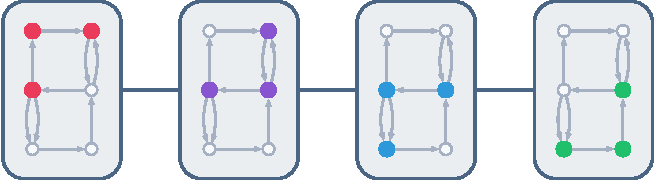
\includegraphics[scale=.5]{ex-tree-dec-full.pdf}%
	}
	\hfill
	\subfloat[``Concise'' representation of $(T, \bagmap)$]{%
		\AP\label{fig:ex-tree-dec-concise}
		
\includegraphics[scale=1.1]{ex-tree-dec-concise.pdf}
	}
	\caption{
		\AP\label{fig:ex-tree-dec}
		Two different representations of the same "tree decomposition" $(T, \bagmap)$ of a 
		multigraph $G$ with six 
		vertices. The underlying tree is a path with four nodes and each "bag" contains 3 
		vertices---hence the "decomposition@tree decomposition" has "width" 2.
	}
\end{figure}
We give an example of "tree decomposition" in \Cref{fig:ex-tree-dec}:
\begin{itemize}
	\item In \Cref{fig:ex-tree-dec-full}, we give the ``full'' representation of
	the "decomposition@tree decomposition": we draw $T$, and inside each "bag" $b$ of $T$
	we represent a copy of $G$. Nodes of $G$ belonging to $b$ are highlighted, while the others are dimmed. Sometimes, we will only write the
	name of the nodes contained in the "bag", instead of drawing the graph.
	\item In \Cref{fig:ex-tree-dec-concise}, we give a ``concise'' representation:
	we draw over $G$ a coloured shape for each "bag" of $T$. This representation is ambiguous---the structure of $T$ is not made explicit---and will only be used when no ambiguity can arise.
\end{itemize}

The \AP""tree-width"" of $G$ is the minimum of the "width" of all "tree decompositions" of $G$. The \reintro{tree-width} of a "C2RPQ" is the "tree-width" of its underlying multigraph. 
We denote by $\intro*\Tw$ (resp.\ $\intro*\TwOneWay$) the set of all "C2RPQs" (resp.\ "CRPQs") of "tree-width" at most $k$. The \reintro{tree-width} of a "UC2RPQ" is simply the maximum of the "tree-width" of its "C2RPQs".
\AP
A ""path decomposition"" is a "tree decomposition" $(T,\bagmap)$ in which $T$ is a path. The \AP""path-width"" of $\gamma$ is the minimum of the "width" among all "path decompositions" of $\gamma$. The \reintro{path-width} of a "C2RPQ" and "UC2RPQ" are defined analogously. We denote by \AP$\intro*\Pw$ (resp.\ $\intro*\PwOneWay$) the set of all "C2RPQs" (resp.\ "CRPQs") of "path-width" at most $k$. The relationship between these classes is depicted in \Cref{fig:taonomy-syntactic}:
note that $\TwOneWay$ and $\PwOneWay$ are not explicitly drawn, but correspond to the
intersection of $\Tw$ (resp.\ $\Pw$) with the class of "CRPQs".

\begin{figure}
	\centering
	\scalebox{1.125}{
	\begin{tikzpicture}
		\node at (0,0) {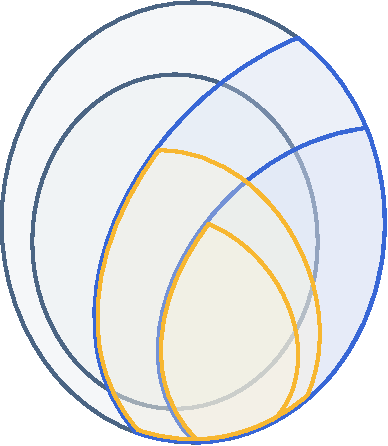
\includegraphics[scale=.8]{taxonomy-syntactic.pdf}};
		% \draw[line width=1.5pt] (0,-4) -- (0,4);
		% \draw[line width=1.5pt] (-3,0) -- (3,0);
		% \draw[line width=.5pt] (1,-4) -- (1,4);
		% \draw[line width=.5pt] (-3,1) -- (3,1);
		% \draw[line width=.5pt] (-1,-4) -- (-1,4);
		% \draw[line width=.5pt] (-3,-1) -- (3,-1);
		\node[font=\small] at (.5,-1.5)
			{$\withkl{\kl[\Pw]}{\cmdkl{\color{cYellow}\mathcal{P\hspace{-.15em}w}_{1\!}}}$};
		\node[font=\small] at (-.5,0) 
			{$\withkl{\kl[\Pw]}{\cmdkl{\color{cYellow}\mathcal{P\hspace{-.15em}w}_{k\!}}}$};
		\node[font=\small] at (2.05,.2)
			{$\withkl{\kl[\Tw]}{\cmdkl{\color{cBlue}\mathcal{T\hspace{-.15em}w}_{1\!}}}$};
		\node[font=\small] at (1.4,1.8)
			{$\withkl{\kl[\Tw]}{\cmdkl{\color{cBlue}\mathcal{T\hspace{-.15em}w}_{k\!}}}$};
		\node[font=\tiny] at (-1.5,.5) {\kl[CRPQ]{\color{cDarkGrey}CRPQs}};
		\node[font=\tiny] at (-.5,2.4) {\kl[C2RPQ]{\color{cDarkGrey}C2RPQs}};
	\end{tikzpicture}
	}
	\caption{
		\AP\label{fig:taonomy-syntactic}
		Clickable taxonomy of syntactic classes studied in this paper.
	}
\end{figure}

% \begin{proposition}[Folklore, see "eg" {\cite[Theorem IV.3]{DBLP:conf/lics/0001BV17}}]
%     For each $k \geq 1$, the "evaluation problem" for "UC2RPQs" of "tree-width" at
%     most $k$ is in polynomial time.\sideremi{Find better ref?}
% \end{proposition}

Similar statements of the following proposition can be considered Folklore (see "eg" {\cite[Theorem IV.3]{DBLP:conf/lics/0001BV17}}); however, our inability to find a proof for it with sharp bounds invites us to include a proof.
\begin{restatable}[Proof in \Cref{apdx-sec:prop:crpq-bound-tree-width-upper-bound}]{prop}{crpqboundtwupperbound}
	\AP\label{prop:crpq-bound-tree-width-upper-bound}
    For each $k \geq 1$, the "evaluation problem" for "UC2RPQs" of "tree-width" at
    most $k$ can be solved in time $\+O(\size{\Gamma} \cdot |G|^{k+1} \cdot \log{|G|})$ on a Turing machine,
	% \sideremi{I've kept both complexities, but made it clear that the first one is about TM. Is it ok?} 
	% \sidediego{yes!}
	or $\+O(\size{\Gamma} \cdot |G|^{k+1})$ under a RAM model, where $\Gamma$ and $G$ are the input "UC2RPQ" and "graph database", respectively.
\end{restatable}



In practice, "graph databases" tend to be huge and often changing, while queries
are in comparison very small.
This motivates the following question, given some natural $k \geq 1$: 

\begin{center}
    \AP 
    Given a "UC2RPQ" $\Gamma$, is it "equivalent" to a "UC2RPQ" $\Gamma'$ of "tree-width" at most $k$?\\
    That is, does it have ""semantic tree-width"" at most $k$?
\end{center}
This problem is called the ""semantic tree-width $k$ problem"".
Should it be decidable in a constructive way---that is, decidable, and if the answer is positive, we can compute a witnessing $\Gamma'$ from $\Gamma$---, then one could, once and for all,
compute $\Gamma'$ from $\Gamma$ and, whenever one wants to "evaluate" $\Gamma$ on a
database, "evaluate" $\Gamma'$ instead.

We will also study the restriction of these notions to one-way queries: a "UCRPQ" has \AP""one-way semantic tree-width"" at most $k$ if it is equivalent to a "UCRPQ" of "tree-width" at most $k$. The \AP""one-way semantic tree-width $k$ problem"" is the problem of, given a "UCRPQ" $\Gamma$, whether it has "one-way semantic tree-width" at most $k$.

\begin{example}
    \AP\label{ex:CRPQ-tw3-stw2}
    Consider the following "CRPQs",\footnote{In this graphical representation,
	we interpret a labelled graph as the "CRPQ" defined as
	the conjunction of the "atoms" induced by the labelled edges of the graph.
	For instance, $\gamma(\bar x)$ is a conjunction of six "atoms".}
    where $\bar x = (x_0,x_1,y,z)$:\leavevmode
    \begin{center}
        \small
        \begin{tikzcd}[column sep=small, row sep=small]
            &[-.5em] x_0 \ar[dr, "a"] \ar[rr, "c"] \ar[ddr, "a(bb)^+" swap, pos=.6, bend right] & &
            x_1 \ar[dl, "a" swap] \ar[ddl, "ab(bb)^*", pos=.7, bend left]
                &[1.5em] &[-.5em] x_0 \ar[dr, "a"] \ar[rr, "c"] \ar[ddr, "a(bb)^+" swap, pos=.6, bend right] & &
                x_1 \ar[dl, "a" swap] 
                    &[1.5em] &[-.5em] x_0 \ar[dr, "a"] \ar[rr, "c"]  & &
                    x_1 \ar[dl, "a" swap] \ar[ddl, "ab(bb)^*", pos=.6, bend left] \\
            \gamma(\bar x) \defeq & & y \ar[d, "b^+", pos=.35] & 
                & \delta(\bar x) \defeq & & y \ar[d, "b(bb)^*" pos=.35] & 
                    & \delta'(\bar x) \defeq & & y \ar[d, "(bb)^+" swap, pos=.35] & \\
            & & z & 
                & & & z & 
                    & & & z &
        \end{tikzcd}
    \end{center}
    \noindent
    The underlying graph of $\gamma(\bar x)$ being the directed 4-clique, $\gamma 
    (\bar x)$ has "tree-width" 3. We claim that $\gamma(\bar x)$ is equivalent to the "UCRPQ"
    $\delta(\bar x) \lor \delta'(\bar x)$, and hence has "one-way semantic tree-width" at most 2.

    Indeed, given a "graph database" satisfying $\gamma(\bar x)$ via some mapping $\mu$, 
    it suffices to make a case disjunction on whether the number of $b$-labelled "atoms"
    in the path from
    $\mu(y)$ to $\mu(z)$ is even or odd. In the first case, the "atom" $x_0\atom{a(bb)^+} z$ becomes
    redundant since we can deduce the existence of such a path from the conjunction
    $x \atom{a} y \atom{(bb)^+} z$, and hence the "database" "satisfies" $\delta(\bar x)$ via $\mu$.
    Symmetrically, in the second case, the "atom" $x_1 \atom{b(bb)^*} z$ becomes redundant,
    and the "database" "satisfies" $\delta'(\bar x)$ via $\mu$. 
    Thus, $\gamma(\bar x)$
    is "contained", and hence "equivalent" (the other "containment" being trivial), to
    the "UCRPQ" $\delta(\bar x) \lor \delta'(\bar x)$ of "tree-width" 2.
\end{example}

\subsection{\AP{}Related Work}
\label{sec:relwork}
On the class "conjunctive queries", the "semantic tree-width $k$ problem" becomes the "coNP"-complete problem of finding out whether the retraction of a query has "tree-width"
at most $k$. In fact, "CQs" enjoy the effective existence of unique minimal queries \cite[Theorem 12]{DBLP:conf/stoc/ChandraM77}, which happen to also minimize the tree-width. For "CRPQs" and "UC2RPQs", the question is far more challenging, and it has only been solved for the case $k = 1$ 
by Barceló, Romero, and Vardi \cite[Theorem 6.1]{BarceloRV16}; the case $k>1$ was left widely open
\cite[\S 7]{BarceloRV16}.

Furthermore, classes of "CQs" of bounded "semantic tree-width" precisely characterize tractable (and "FPT") "evaluation problem" \cite[Theorem~1.1]{Grohe07}.
This result is on bounded-arity schemas, which was later generalized \cite[Theorem~1]{DBLP:conf/ijcai/ChenGLP20} for characterizing "FPT" "evaluation" on arbitrary schemas---by replacing "semantic tree-width" with semantic ``submodular width'' \cite{Marx13}.

The problem of computing "maximal under-approximations" of "CQs" of a given "tree-width" has been explored in \cite{DBLP:journals/siamcomp/BarceloL014}.
A "maximal under-approximations" of tree-width at most $k$ of a "CQ" $\gamma$ consists of a
"CQ" $\delta_k$ of "tree-width" at most $k$, which under-approximates it,
"ie" $\delta_k$ is "contained" in $\gamma$, and which is maximal, in the sense that for every "CQ" 
$\delta'$, if $\delta'$ has "tree-width" at most $k$ and is "contained" in $\gamma$, then 
$\delta'$ is "contained" in $\delta_k$. 
"Maximal under-approximations" of a given "tree-width" for "CQs" always exist \cite{DBLP:journals/siamcomp/BarceloL014} and thus, a "CQ" is "semantically equivalent"
to a "CQ" of "tree-width" at most $k$ if, and only if, it is equivalent to its maximal under-approximation of "tree-width" at most $k$. Our solution to decide the
"semantic tree-width $k$ problem" for "UC2RPQs" is based on this idea.

While "maximal under-approximations" always exist for "CQs", this is not the case for the dual notion of ``minimal over-approximations''. The problem of when these exist is still unknown to be decidable, aside for some the special cases of acyclic "CQs" and Boolean "CQs" over binary schemas \cite{DBLP:journals/mst/BarceloRZ20}.


\subsection{\AP{}Contributions}
% \remi{Please check this subsection. I had to move some paragraphs around ("closed under sublanguages") was defined after its first use.}
Here we solve both the "semantic tree-width $k$ problem" and "one-way semantic tree-width $k$ problem" for every $k$ with one unifying approach.
\begin{theorem}
    \AP\label{thm:decidability-semtw}
    For each $k \geq 1$, the "semantic tree-width $k$ problem" and the "one-way semantic tree-width $k$ problem" are decidable. Moreover, these problems are in "2ExpSpace" and are "ExpSpace"-hard.
	When $k=1$, the problems are in fact "ExpSpace"-complete.
\end{theorem}
In \Cref{sec:maximal-under-approximations} (\Cref{lem:sem-tw-in-twoexp}),
we prove the upper bound for $k\geq 2$, by relying on the so-called ``"Key Lemma"'', which is our main technical result, and is proven in \Cref{sec:treedec,sec:proof-key-lemma}.
The upper bound for the case $k=1$---which was already proven in \cite{BarceloRV16} for the (two-way) "semantic tree-width $1$ problem"---is shown in \Cref{sec:acyclic-queries} (\Cref{cor:sem-tw-1-pb-exp-c}). The lower bound is shown in \Cref{sec:lowerbound} (\Cref{lemma:lowerbound}).

The "Key Lemma" (\Cref{lemma:bound_size_refinements}) essentially states that
every "UC2RPQ" has a computable ``maximal under approximation'' by a "UC2RPQ" of "tree-width" $k$ and that this approximation is well-behaved with respect to the class of languages used to label the queries under some mild assumptions on it (being ``"closed under sublanguages"''). Let us first
explain this assumption before formalizing the statement above (stated as \Cref{cor:mua-exists-effective}).

For a class $\+L$ of languages, let $\intro*\UCtwoRPQ(\+L)$ denote the class of all "UC2RPQs" whose atoms are all labelled by languages from $\+L$.
\AP For an NFA $\+A$ and two states $q,q'$ thereof, we denote by $\intro*\subaut{\+A}{q}{q'}$ the ""sublanguage"" of $\+A$ recognized  when considering $\set{q}$ as the set of initial states and $\set{q'}$ as the set of final states.
\AP We say that $\+L$ is ""closed under sublanguages"" if
(i) it contains every language of the form $\{a\}$,
where $a \in \A$ is any (positive) letter such that either $a$ or $a^-$ occur in a word of a
language of $\+L$, and (ii) for every language $L \in \+L$ there exists an NFA $\+A_L$ accepting $L$ such that every "sublanguage" $\subaut{\+A_L}{q}{q'}$ distinct from $\emptyset$ and
$\{\varepsilon\}$ belongs to $\+L$.

To the best of our knowledge,
all classes of regular expressions that have been considered in the realm of regular path queries (see, "eg", \cite[\S1]{FigueiraGKMNT20}) are "closed under sublanguages". In particular, this is
the case for the class $\bigl\{ \{a_1+\hdots+a_n\} \mid a_1,\hdots,a_n
\in \A \bigr\} \cup \bigl\{ a^* \mid a \in \A \bigr\}$, which will be our focus of study in \Cref{sec:sre}. Moreover, even if some class $\+L$
is not "closed under sublanguages", such as $\{(aa)^*\}$,
then it is contained in a minimal class "closed under sublanguages"---$\{a, a(aa)^*, (aa)^*\}$ in 
this example.

We can now state the main implication of the "Key Lemma" (whose formal statement requires some extra definitions).
\begin{restatable*}[Existence of the "maximal under-approximation"]{cor}{muaexistseffective}
    \AP\label{cor:mua-exists-effective}
    % Fix $k > 1$ and a class $\+L$ of regular languages closed under "sublanguages". Then, every $\UCtwoRPQ(\+L)$ query has a 
    % "maximal under-approximation" by infinitary unions of $\Tw$ queries that can be effectively computed as a $\UCtwoRPQ(\+L)$ query in "ExpSpace".
    For each $k \geq 2$, for each class $\+L$ "closed under sublanguages",
    and for each query $\Gamma \in \UCtwoRPQ(\+L)$,
    there exists $\Gamma' \in \UCtwoRPQ(\+L)$ of "tree-width" at most $k$ 
    such that
    $\Gamma' \contained \Gamma$, and for every $\Delta \in \UCtwoRPQ$, if $\Delta$ has
    "tree-width" at most $k$ and $\Delta \contained \Gamma$, then $\Delta \contained \Gamma'$.
    Moreover, $\Gamma'$ is computable from $\Gamma$ in "ExpSpace".
\end{restatable*}

As a consequence of \Cref{cor:mua-exists-effective,prop:crpq-bound-tree-width-upper-bound}, we have that queries of bounded "semantic tree-width" have tractable evaluation.
\begin{restatable*}[FPT evaluation for bounded "semantic tree-width"]{cor}{fptEvalBoundedSemTreeWidth}
	\AP\label{coro:fpt-eval-bounded-semtreewidth}
	For each $k\geq 1$, the "evaluation problem" for "C2RPQs" of "semantic tree-width"
	at most $k$ is fixed-parameter tractable---"FPT"---when parametrized in the size of
	the query. More precisely on input $\langle \Gamma, G \rangle$,
	the algorithm runs in time
	$\+O(f(\size{\Gamma})\cdot |G|^{k+1} \cdot \log{|G|})$ on a Turing machine, where $f$ is a doubly-exponential function---or $\+O(f(\size{\Gamma})\cdot |G|^{k+1})$ under a RAM model.
\end{restatable*}
Note that \cite[Theorem~22]{FGM24} shows that the statement above can be improved to have a single-exponential function $f$.

% Essentially, this means that to minimize the "semantic tree-width" of a query, we do not need to ``create'' new languages.
% 138/139 and 153/154: It took me a while to see why this does not follow from the definition. It 
% would have helped me, if there was an informal pointer that semantic acyclicity always refers 
% to 2-way CRPQs (for understanding this I also looked at Barcelo/Romero/Vardi,
% there it also took me a moment).
% In other words, if a query
% can be defined with labels in $\+L$, and if this query is equivalent to a  
% query of small tree-width, then it is also equivalent to a query of small tree-width
% with labels in $\+L$.
% In particular, for any $k>1$, a "CRPQ" is equivalent to a "UC2RPQ" of "tree-width" at most $k$ if{f} it is e equivalent to "UCRPQ" of "tree-width" at most $k$, which is not true for $k=1$ ("cf" \Cref{rk:closure-under-sublanguages-k1}, also \cite[Proposition 6.4]{BarceloRV16}).

Moreover, we also show that for any class $\+L$ of regular languages "closed under sublanguages", if $\Gamma \in \UCtwoRPQ(\+L)$ has "semantic tree-width" $k > 1$,
then $\Gamma$ is equivalent to a $\UCtwoRPQ(\+L)$ of "tree-width" at most $k$.
Analogous characterizations hold for $k=1$ and/or "path-width", see \Cref{coro:charact-semantic-treewidth-1,coro:charact-semantic-pathwidth-k}.

\begin{restatable*}{thm}{closureundersublanguages}
    \AP\label{thm:closure-under-sublanguages}
    \AP Assume that $\+L$ is "closed under sublanguages". 
    For any $k > 1$ and any query $\Gamma \in \UCtwoRPQ(\+L)$, the following are equivalent:
    \begin{enumerate}
        \itemAP[\introinrestatable{\itemClosureInfCQ}] $\Gamma$ is "equivalent" to an "infinitary union" of "conjunctive queries"
            of "tree-width" at most $k$; \label{thm:closure-under-sublanguages:1}
        \itemAP[\introinrestatable{\itemClosureUCRPQ}] $\Gamma$ has "semantic tree-width" at most $k$; \label{thm:closure-under-sublanguages:2}
        \itemAP[\introinrestatable{\itemClosureUCRPQSimple}] $\Gamma$ is "equivalent" to a $\UCtwoRPQ(\+L)$ of "tree-width" at most $k$. \label{thm:closure-under-sublanguages:3}
    \end{enumerate}
\end{restatable*}

The implications $\itemClosureUCRPQSimple \Rightarrow \itemClosureUCRPQ \Rightarrow \itemClosureInfCQ$ immediately follow
from the definition of the "semantic tree-width".
On the other hand, the
implications $\itemClosureInfCQ \Rightarrow \itemClosureUCRPQ$ and $\itemClosureUCRPQ \Rightarrow \itemClosureUCRPQSimple$ are surprising,
since they are both trivially false when $k=1$. We defer the proof of this last claim
to \Cref{rk:closure-under-sublanguages-k1} as we first need a few tools to manipulate "CRPQs".

% The proof of our "key lemma" spans over
% \Cref{sec:approximations,sec:treedec,sec:proof-approximations}:
% in \Cref{sec:approximations}, we introduce necessary notions to formally state it,
% and deduce \Cref{thm:decidability-semtw,thm:closure-under-sublanguages} from it;
% in \Cref{sec:treedec} we introduce the central notion of "tagged tree decompositions"
% of "C2RPQs homomorphisms", and building on it, we finally describe the
% constructions used to prove the "Key Lemma" in \Cref{sec:proof-approximations}.

The previous theorem, together with the high complexity of "semantic tree-width $k$ problem",
motivates us to focus on the case of "CRPQs" using some "simple regular expressions" ("SRE") in \Cref{sec:sre}, where we show that the complexity of this problem is much lower.
% coincides with the complexity of the "containment problem" over this class of "CRPQs" \cite[Corollary~5.2]{FigueiraGKMNT20}:

\begin{restatable*}{thm}{thmSemTwSREpitwo}
    \AP\label{thm:semtw-sre-pitwo}
    For $k\geq 2$, the "semantic tree-width $k$ problem" for {\UCRPQSRE} is in "Pi2".
\end{restatable*}

We then study the problem of $k=1$: at first glance, our proof for $k\geq 2$ of
\Cref{thm:decidability-semtw} does not capture this case, for a technical---yet crucial---reason. In
\Cref{sec:acyclic-queries}, we explain how to adapt our proof to capture it: 
and show the decidability the "semantic tree-width 1 problem"---which was already studied by 
Barceló, Romero and Vardi \cite{BarceloRV16}---and of the "one-way semantic tree-width 1 problem". 

Building on the same idea, we show in \Cref{sec:semantic-path-width} that our results extend to "path-width".
\begin{restatable*}{thm}{decidabilitySemPw}
    \AP\label{thm:decidability-sempw}
    For each $k \geq 1$,
    the "semantic path-width $k$ problems" are decidable. Moreover, they lie in "2ExpSpace"
    and are "ExpSpace"-hard. Moreover, if $k=1$, these problems are in fact "ExpSpace"-complete.
\end{restatable*}
In turn, this leads to an evaluation algorithm with a remarkably low complexity.
\begin{restatable*}{thm}{paraNLEvalBoundedSemPathWidth}
	\AP\label{thm:evaluation-bounded-pathwidth}
	For each $k \geq 1$, the "evaluation problem", restricted to "UC2RPQs" of
	"semantic path-width" at most $k$ is in "para-NL" when parametrized in the size of the query.
	More precisely, the problem, on input $\langle \Gamma, G \rangle$, can be solved in
	non-deterministic space $f(|\Gamma|) + \log(|G|)$, where $f$ is a single exponential
	function.
\end{restatable*}

\begin{figure}
	\centering
	\subfloat[Semantic classes of "C2RPQs" related to "tree-width".]{
		\AP\label{fig:taxonomy-semantic-tw}
		\scalebox{1.125}{
		\begin{tikzpicture}
			\node at (0,0) {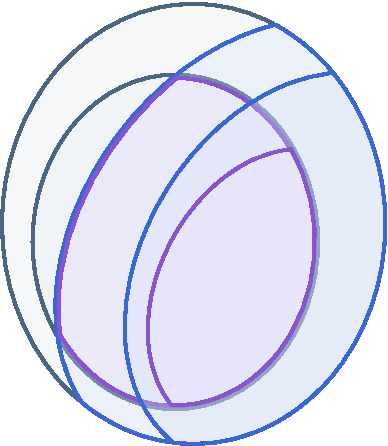
\includegraphics[scale=.8]{taxonomy-semantic-tw.pdf}};
			% \draw[line width=1.5pt] (0,-4) -- (0,4);
			% \draw[line width=1.5pt] (-3,0) -- (3,0);
			% \draw[line width=.5pt] (1,-4) -- (1,4);
			% \draw[line width=.5pt] (-3,1) -- (3,1);
			% \draw[line width=.5pt] (-1,-4) -- (-1,4);
			% \draw[line width=.5pt] (-3,-1) -- (3,-1);
			\node[font=\tiny, align=center] at (.6,-.7)
				{\kl[one-way semantic tree-width]{\color{cPurple}1way sem.}\\ \kl[one-way semantic tree-width]{\color{cPurple}tw 1}};
			\node[font=\tiny, align=center] at (-1,.3)
				{\kl[one-way semantic tree-width]{\color{cPurple}1way}\\ \kl[one-way semantic tree-width]{\color{cPurple}sem.}\\ \kl[one-way semantic tree-width]{\color{cPurple}tw $k$}};
			\node[font=\tiny, align=center] at (1.9,.9)
				{\kl[semantic tree-width]{\color{cBlue}sem.}\\ \kl[semantic tree-width]{\color{cBlue}tw 1}};
			\node[font=\tiny, align=center] at (1,2.2)
				{\kl[semantic tree-width]{\color{cBlue}sem.}\\ \kl[semantic tree-width]{\color{cBlue}tw $k$}};
			\node[font=\tiny] at (-1.6,.8) {\kl[CRPQ]{\rotatebox{60}{\color{cDarkGrey}CRPQs}}};
			\node[font=\tiny] at (-.5,2.4) {\kl[C2RPQ]{\color{cDarkGrey}C2RPQs}};
		\end{tikzpicture}
		}
	}
	\hfill
	\subfloat[Semantic classes of "C2RPQs" related to "path-width".]{
		\AP\label{fig:taxonomy-semantic-pw}		
		\centering 
		\scalebox{1.125}{
		\begin{tikzpicture}
			\node at (0,0) {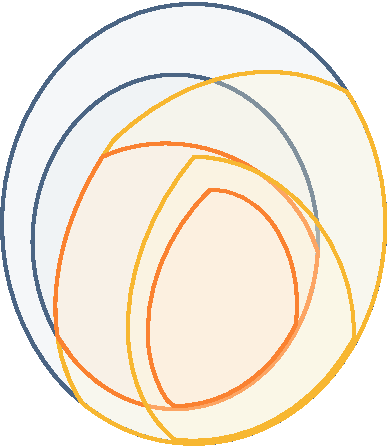
\includegraphics[scale=.8]{taxonomy-semantic-pw.pdf}};
			% \draw[line width=1.5pt] (0,-4) -- (0,4);
			% \draw[line width=1.5pt] (-3,0) -- (3,0);
			% \draw[line width=.5pt] (1,-4) -- (1,4);
			% \draw[line width=.5pt] (-3,1) -- (3,1);
			% \draw[line width=.5pt] (-1,-4) -- (-1,4);
			% \draw[line width=.5pt] (-3,-1) -- (3,-1);
			\node[font=\tiny, align=center] at (.4,-1)
				{\kl[one-way semantic path-width]{\color{cOrange}1way sem.}\\ \kl[one-way semantic path-width]{\color{cOrange}pw 1}};
			\node[font=\tiny, align=center] at (-1.1,0)
				{\kl[one-way semantic path-width]{\color{cOrange}1way}\\ \kl[one-way semantic path-width]{\color{cOrange}sem.}\\ \kl[one-way semantic path-width]{\color{cOrange}pw $k$}};
			\node[font=\tiny] at (1,-2.35) {\kl[semantic path-width]{\rotatebox{33}{\color{cYellow}sem. pw 1}}};
			\node[font=\tiny, align=center] at (1.9,.9)
				{\kl[semantic path-width]{\color{cYellow}sem.}\\ \kl[semantic path-width]{\color{cYellow}pw $k$}};
			\node[font=\tiny] at (-1.6,.8) {\kl[CRPQ]{\rotatebox{60}{\color{cDarkGrey}CRPQs}}};
			\node[font=\tiny] at (-.5,2.4) {\kl[C2RPQ]{\color{cDarkGrey}C2RPQs}};
		\end{tikzpicture}
		}
	}
	\caption{
		\AP\label{fig:taxonomy-semantic}
		Clickable taxonomy of semantic classes studied in this paper, where $k \geq 2$.
	}
\end{figure}
Interestingly, the proof for "tree-width" 1 and "path-width" $k$ ($k \geq 1$)
can be derived from the proof from "tree-width" $k\geq 2$ but necessitates an
additional technical trick which yields different closure properties (or lack thereof).
We show that a "UCRPQ" has "semantic tree-width" at most $k$ if, and only if, it
has "one-way semantic tree-width" at most $k$ whenever $k \geq 2$
(\Cref{coro:collapse-twoway-oneway-semtw}). In other words, if the original query does not
use "two-way navigation", then considering "UC2RPQs" does not help to further minimize the "tree-width". Interestingly, this is false for $k=1$ ("cf" \Cref{rk:closure-under-sublanguages-k1},
also \cite[Proposition 6.4]{BarceloRV16}) and for "path-width", no matter the value of $k\geq 1$ (see \Cref{rk:path-width:oneway-vs-twoway}). Overall, this leads to
the landscape depicted in \Cref{fig:taxonomy-semantic}.

Finally, we conclude in \Cref{sec:discussion}.
We provide a \emph{partial} characterization \emph{à la} Grohe of classes of "UC2RPQs" which admit a tractable evaluation in \Cref{sec:charact-tractability}.
\begin{restatable*}{thm}{thmtractabilityfinred}
    \AP\label{thm:tractability-finred}
    Assuming $"W[1]" \neq $ "FPT", for any recursively enumerable class $\+C$ of "finitely-redundant" Boolean "UC2RPQs", the "evaluation problem" for $\+C$ is "FPT" if, and only if, $\+C$ has bounded "semantic tree-width".
\end{restatable*}
We also discuss open questions, ranging from complexity
questions (\Cref{sec:discussion-complexity}) to extensions of our results to bigger classes
or larger settings (\Cref{sec:discussion-larger-classes,sec:discussion-different-notions}).

% \subsection{\AP{}Conference Paper}
% \label{sec:conf-paper-diff}
% The current article is based on the conference paper \cite{thispaperICDT}. The main results for "tree-width" $k>1$ are essentially the same---though with improved explanations and figures, and we fixed some minor bugs in the proof of the "Key Lemma". Here we also show how to extend our techniques to tackle the "semantic tree-width $1$ problem" (\Cref{sec:acyclic-queries}) and we introduce and study the "semantic path-width $k$ problems" (\Cref{sec:semantic-path-width}). Our very partial lift of Grohe's characterization of "FPT" classes of queries (\Cref{thm:tractability-finred}) is also new.